\section{Dynamic analysis}

Testing serves the purpose of analyzing the behavior of programs.
In this context, properties are translated into executable oracles, serving as representations of anticipated outputs and desired conditions.
The primary limitation of testing lies in its reliance on a finite set of test cases, rendering this form of verification non-exhaustive. 
Failures manifest with specific inputs that act as triggers, and the execution process is automated.
It is crucial to recognize that the primary objective of testing is to uncover program failures. 
Other common goals include:
\begin{itemize}
    \item Exercising different segments of a program to enhance coverage.
    \item Verifying the seamless interaction between components (integration testing).
    \item Facilitating fault localization and error removal (debugging).
    \item Ensuring that previously introduced bugs do not resurface (regression testing).
\end{itemize}

\paragraph*{Test cases}
A test case comprises a collection of inputs, execution conditions, and a criterion for determining pass or fail outcomes.
The typical sequence for executing a test case involves:
\begin{itemize}
    \item \textit{Setup}: establish the initial state of the program to meet specified execution conditions.
    \item \textit{Execution}: execute the program using the provided inputs.
    \item \textit{Teardown}: document the output, final state, and any failures identified based on the pass/fail criterion.
\end{itemize}
A testing suite, encompassing numerous test cases, can be employed for comprehensive evaluation. 
The specification of a test case outlines the requirements to be met by one or more actual test cases.

\paragraph*{Unit testing}
Developers perform unit testing, focusing on examining isolated, small sections (units) of code. 
The definition of a unit is often influenced by the programming language in use. 
Unit testing serves to identify issues at an early stage, provides guidance in design, and enhances overall code coverage.
However, a challenge in testing isolation arises due to potential dependencies between units. 
To address this, a viable solution involves simulating the absent units.

\subsection{Integration testing}
Integration testing is focused on validating the interaction and interfaces among components.
The potential faults uncovered during integration testing include:
\begin{itemize}
    \item Inconsistent interpretation of parameters.
    \item Violations of assumptions about domains.
    \item Side effects on parameters or resources.
    \item Nonfunctional properties.
\end{itemize}
Integration and testing plans are typically outlined in the Design Document. 
The build plan dictates the implementation order, while the test plan details the execution of integration testing. 
Ensuring the test plan aligns with the build plan is crucial.
The most commonly employed strategies for integration testing are:
\begin{itemize}
    \item \textit{Big bang}: testing occurs only after integrating all modules together. 
        This strategy has the advantage of not requiring stubs and needing fewer drivers and oracles. 
        However, it has drawbacks such as minimal observability, challenging fault localization, reduced efficacy, and delayed feedback. 
        The cost of repairing faults found in later stages is also high.
    \item \textit{Iterative and incremental strategies}: Tests are run as soon as components are released. 
        This approach is structured around the hierarchical system design, leading to the following techniques:
        \begin{itemize}
            \item \textit{Top-down strategy}: progressing from the top level in terms of use or include relation.
                Drivers use top-level interfaces, but the need for stubs at each step can be a challenge. 
                As modules are ready (following the build plan) more functionality is testable.
                As modules become available following the build plan, more functionality becomes testable, with stubs gradually replaced.
            \item \textit{Bottom-up strategy}: starting from the leaves of the uses hierarchy, this strategy doesn't require stubs.
                However, more drivers are typically needed (one for each module, similar to unit testing). 
                It may result in multiple working subsystems that are eventually integrated into the final one.
            \item \textit{Threads strategy}: integrating portions of several modules that collectively offer a user-visible function. 
                This approach minimizes the need for drivers and stubs but introduces complexity to the integration plan.
            \item \textit{Critical modules strategy}: commencing with modules carrying the highest risk, this strategy may resemble a threaded process with specific priorities. 
                The focus is on a risk-oriented process, treating integration and testing as proactive measures to identify issues early.
        \end{itemize}
\end{itemize}

\paragraph*{Strategy selection}
Structural strategies, such as bottom-up and top-down, offer simplicity. 
In contrast, thread and critical modules strategies enhance external visibility of progress, especially in complex systems. 
It is viable to combine different strategies based on the specific requirements.
Top-down and bottom-up strategies are suitable for relatively small components and subsystems.
On the other hand, combinations of thread and critical modules integration testing are often preferred when dealing with larger subsystems. 
The selection of strategies depends on the nature and scale of the system under consideration.

\subsection{System testing}
End-to-end testing of the entire integrated system is carried out by independent teams, with the testing environment closely resembling the production setup. 
This testing encompasses both functional and non-functional aspects.
Key strategies employed in system end-to-end testing include:
\begin{itemize}
    \item \textit{Functional testing}: verifying if the software aligns with functional requirements, this involves using the software according to use cases outlined in the RASD and checking for fulfillment of requirements.
    \item \textit{Performance testing}: identifying bottlenecks affecting response time, utilization, and throughput.
        It detects inefficient algorithms, hardware, or network issues and suggests optimizations. 
        The system is loaded with the expected workload to ensure the measured performance aligns with expectations.
    \item \textit{Load testing}: exposing issues like memory leaks, memory mismanagement, and buffer overflows, load testing determines the upper limits of system components and compares alternative architectural options. 
        The system is tested under increasing workloads until it reaches its capacity, and the load is sustained over an extended period.
    \item \textit{Stress testing}: ensuring graceful recovery after failure, stress testing aims to break the system under test by overwhelming its resources or by reducing available resources.
\end{itemize}
\begin{figure}
    \centering
    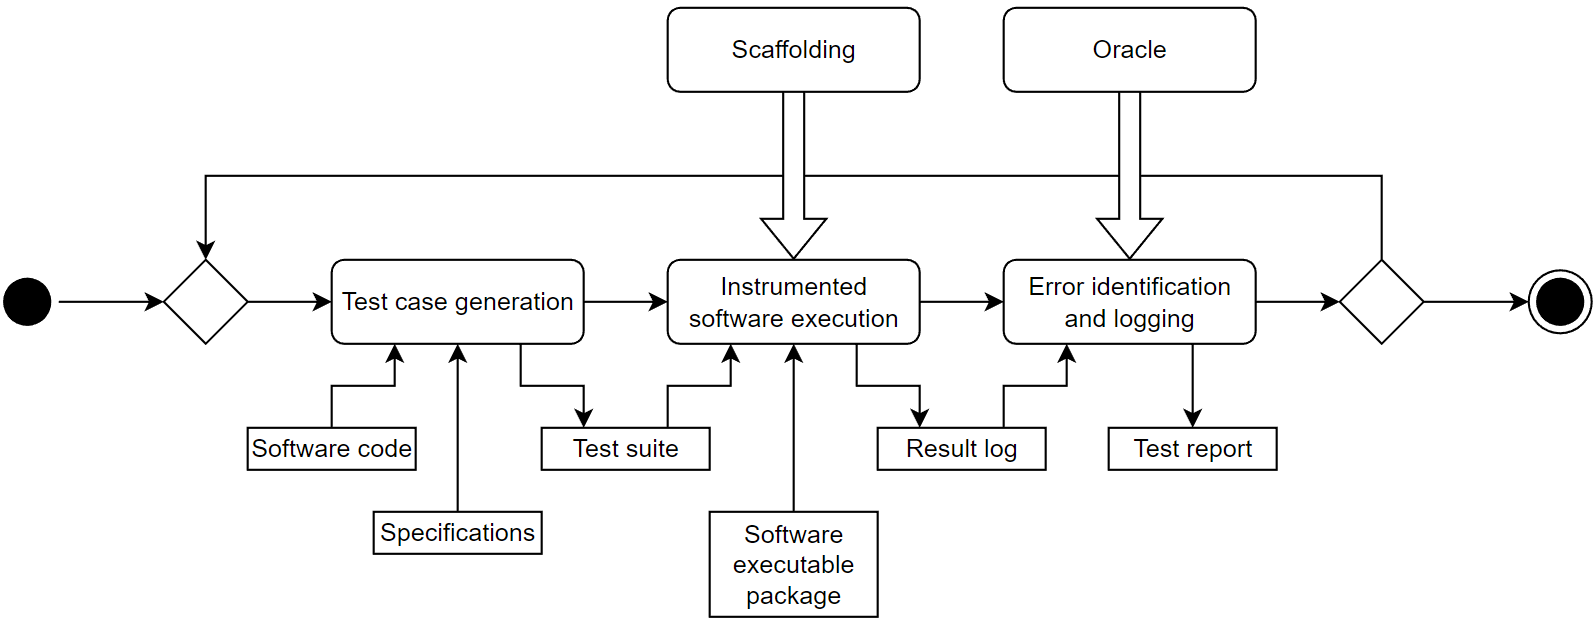
\includegraphics[width=0.75\linewidth]{images/twf.png}
    \caption{Testing workflow}
\end{figure}

\subsection{Test case generation}
Our objective is to establish high-quality test sets, characterized by:
\begin{itemize}
    \item Demonstrating a high probability of error detection.
    \item Covering an acceptable range of cases.
    \item Maintaining sustainability with a limited number of tests.
\end{itemize}
Test cases can be formulated manually or automatically generated through automated testing techniques, including:
\begin{itemize}
    \item \textit{Combinatorial testing}: enumerating all possible inputs based on a specified policy.
    \item \textit{Concolic execution}: pseudo-random generation of inputs guided by symbolic path properties.
    \item \textit{Fuzz testing (fuzzing)}: pseudo-random generation of inputs, encompassing invalid and unexpected inputs.
    \item \textit{Search-based testing}: exploring the space of valid inputs to identify those improving specific metrics.
\end{itemize}

\paragraph*{Concrete symbolic execution}
Concolic execution involves performing symbolic execution alongside a concrete one, where the state combines a symbolic part and a concrete part. 
These components are used interchangeably to advance exploration. 
The technique involves two steps:
\begin{enumerate}
    \item \textit{Concrete to symbolic}: deriving conditions to explore new paths.
    \item \textit{Symbolic to concrete}: simplifying conditions to generate concrete inputs.
\end{enumerate}
\begin{example}
    \begin{lstlisting}[style=Java]
void m(int x, int y) {
    int z := 2 * y
    if (z == x) {
        z := y + 10
    if (x <= z)
        print(z)
    }
}
    \end{lstlisting}
    We initiate by considering line zero, assigning random variables to $x$ and $y$:
    \begin{table}[H]
        \centering
        \begin{tabular}{l|ccc}
        \textbf{Symbolic state}  & $x$ & $y$ & \multirow{3}{*}{$\left\langle 0 \right\rangle $} \\ \cline{1-3}
        \textbf{Symbolic values} & $X$ & $Y$ &                    \\
        \textbf{Example values}  & $22$ & $7$ &                    
        \end{tabular}
    \end{table}
    Applying this method until the function returns, we obtain:
    \begin{table}[H]
        \centering
        \begin{tabular}{l|ccccc}
        \textbf{Symbolic state}  & $x$ & $y$ & $z$ & $\pi$ & \multirow{3}{*}{$\left\langle 0,1,2,6,7 \right\rangle $} \\ \cline{1-5}
        \textbf{Symbolic values} & $X$ & $Y$ & $2Y$ & $2Y \neq X$  &                 \\
        \textbf{Example values}  & $22$ & $7$ & $14$ &                  
        \end{tabular}
    \end{table}
    To explore another path, negate the path condition, obtaining the constraint $2Y = X$. 
    Reapplying the procedure with values satisfying the constraint, we obtain:
    \begin{table}[H]
        \centering
        \begin{tabular}{l|ccccc}
        \textbf{Symbolic state}  & $x$ & $y$ & $z$ & $\pi$ & \multirow{4}{*}{$\left\langle 0,1,2,3,4,5,6,7 \right\rangle $} \\ \cline{1-5}
        \textbf{Symbolic values} & $X$ & $Y$ & $2Y$ & \makecell{$2Y = X$ \\ $X \leq Y+10$} &                 \\
        \textbf{Example values}  & $1$ & $2$ & $2$ &                  
        \end{tabular}
    \end{table}
    To explore another path, we negate the second constraint while maintaining the preceding one. 
    The final table in this case is:
    \begin{table}[H]
        \centering
        \begin{tabular}{l|ccccc}
        \textbf{Symbolic state}  & $x$ & $y$ & $z$ & $\pi$ & \multirow{4}{*}{$\left\langle 0,1,2,3,4,6,7 \right\rangle $} \\ \cline{1-5}
        \textbf{Symbolic values} & $X$ & $Y$ & $2Y$ & \makecell{$2Y = X$ \\ $X > Y+10$} &                 \\
        \textbf{Example values}  & $30$ & $15$ & $25$ &                  
        \end{tabular}
    \end{table}
    The final result is that we explored three different paths with three sets of values:
    \begin{itemize}
        \item $\left\langle 0,1,2,6,7 \right\rangle \textnormal{ with values } \{x=22, y=7\}$.
        \item $\left\langle 0,1,2,3,4,5,6,7 \right\rangle \textnormal{ with values } \{x=2, y=1\}$.
        \item $\left\langle 0,1,2,3,4,6,7 \right\rangle \textnormal{ with values } \{x=30, y=15\}$.
    \end{itemize}
\end{example}
The advantages of concolic execution are: 
\begin{itemize}
    \item \textit{Handling black-box functions}: can handle black-box functions within path conditions, which is not achievable with pure symbolic execution.
    \item \textit{Automatic test case generation}: capable of automatically generating concrete test cases based on a specified code coverage criterion.
\end{itemize} 
The limitations are: 
\begin{itemize}
    \item \textit{Fault occurrence limited to specific inputs}: faults may be associated with specific inputs, making it challenging to identify them if they are rare events. 
        Concolic execution might not effectively highlight such issues.
    \item \textit{Path explosion}: the number of paths tends to explode, especially in the presence of complex nested conditions, creating a vast search space. 
        This can lead to challenges in scalability and efficiency.
    \item \textit{Exploration guidance}: lacks a mechanism to guide the exploration systematically; it explores possible paths one by one within the allocated budget, potentially missing efficient exploration strategies.
\end{itemize}

\paragraph*{Fuzzing}
Functional testing and fuzzing are complementary approaches in testing software components or systems, addressing not only correctness but also external qualities such as reliability and security.
Fuzzing, a technique that operates at the component or system level, is particularly effective in uncovering defects that may elude other testing methods due to its use of random and often unexpected inputs.
The core concept of fuzzing involves generating random inputs to observe their impact on the system. 
\begin{example}
    Let's assume we want to fuzz an existing program, such as \texttt{bc}. 
    \texttt{bc} is a UNIX utility serving as a basic calculator, dependent on a character stream denoting mathematical expressions for input.
    We assess the resilience of \texttt{bc} by applying an unpredictable input stream through the following steps:
    \begin{itemize}
        \item Develop a fuzzer: a program designed to produce a random character stream.
        \item Employ the fuzzer to test \texttt{bc} with the aim of identifying vulnerabilities or breaking points.
    \end{itemize}
\end{example}
\begin{definition}[\textit{Fuzz input}]
    A fuzz input s characterized by its randomness and lack of structure. 
\end{definition}
Testing involves creating a substantial input file and assessing the program's behavior based on error messages, crashes, and the presence of illegal characters.
Common errors detected through fuzzing include buffer overflows, missing error checks, and unexpected behavior caused by unconventional input values. 
To enhance the effectiveness of fuzzing, it is advisable to integrate it with runtime memory checks. 
Instrumentation at runtime monitors every memory operation, identifying potential violations such as out-of-bounds accesses, use-after-free, and double-free conditions. 
While this combination may introduce some performance overhead, it streamlines the developer's efforts in identifying and addressing issues.

However, a challenge arises when many programs expect inputs in specific formats. 
Random inputs might have a low probability of exploring deep paths within the program.
To address this, mutational fuzzing can be employed, where existing valid inputs are mutated rather than generating entirely random inputs. 
This approach, guided by coverage information, focuses on evolving successful test cases. 
The fuzzer maintains a population of successful inputs, retaining and mutating those that lead to new paths, thereby improving the exploration of the program's functionality.